\chapter{Results and Discussion}
\label{Results}
% Output screenshots, graphs, or tables
% Performance analysis and comparison
% Challenges faced and solutions
\section{Results}
The following objectives were achieved through the course of this project:
\begin{itemize}
    \item Package Assignment: The project aims to implement a package assignment system that efficiently allocates deliveries to available employees. The assignment algorithm considers factors such as package locations, employee availability and workload distribution to optimize efficiency. By ensuring balanced package distribution, the system enhances delivery management and reduces delays.
    \item Route Optimization: The project integrates an intelligent route optimization system that employs the Greedy Algorithm to determine the efficient delivery paths for employees.  The algorithm minimizes travel time and fuel consumption. The system continuously updates routes based on delivery progress, ensuring adaptive and efficient navigation. By optimizing travel sequences, the system improves delivery speed and overall operational efficiency.
\end{itemize}
\subsection{Login \& Registration Page}
The Login \& Registration Page allows companies and employees to securely create accounts and access the system using Firebase Authentication. It ensures user verification, maintaining session states for seamless navigation.
\begin{center}
    \begin{minipage}{0.45\textwidth}
        \centering
        \includegraphics[width=\linewidth]{6/login.jpg}
        \captionof{figure}{Company Login Page}
    \end{minipage}
    \hfill
    \begin{minipage}{0.45\textwidth}
        \centering
        \includegraphics[width=\linewidth]{6/registration.jpg}
        \captionof{figure}{Company Registration Page}
    \end{minipage}
    
    \vspace{1cm} % Adds space before the third image
    
    \begin{minipage}{0.3\textwidth}  % Adjusted width for consistency
        \centering
        \includegraphics[width=\linewidth]{6/Mobile_login.jpg}
        \captionof{figure}{Delivery Personnel Page}
    \end{minipage}
\end{center}
\subsection{Package \& Employee Details Page}
Package Details: Displays information about uploaded packages, including destination, weight and qr code ensuring efficient assignment.
\\
Employee Details: Lists registered employees with availability status, allowing companies to allocate deliveries effectively.
\begin{center}
    \begin{minipage}{0.45\textwidth}
        \centering
        \includegraphics[width=\linewidth]{6/package_details.jpg}
        \captionof{figure}{Package Details Page}
    \end{minipage}
    \hfill
    \begin{minipage}{0.45\textwidth}
        \centering
        \includegraphics[width=\linewidth]{6/employee_details.jpg}
        \captionof{figure}{Employee Details Page}
    \end{minipage}
\end{center}
\subsection{QR Code Scanning Page}
The system enables companies to generate QR codes for packages, allowing employees to scan them for quick retrieval of delivery details. This feature ensures efficient tracking, reduces manual errors and enhances the overall package management process.

\begin{figure}[H]
\centering
\begin{minipage}{0.24\textwidth}
    \centering
    \includegraphics[width=\linewidth]{6/qr1.jpg}
    \label{fig:qr1}
\end{minipage}%
\hspace{5mm}
\begin{minipage}{0.24\textwidth}
    \centering
    \includegraphics[width=\linewidth]{6/qr2.jpg}
    \label{fig:qr2}
\end{minipage}
\caption{QR Code Scanning}
\label{fig:qrcodes1}
\end{figure}
\subsection{Route Optimization \& Navigation Page}
Route Optimization: Utilizes the Greedy Algorithm and Google Maps API to calculate the efficient delivery routes, minimizing travel distance and time.
\\
Navigation Page: Provides real-time tracking for delivery personnel, ensuring smooth and timely deliveries.
\begin{figure}[H]
\centering
\begin{minipage}{0.24\textwidth}
    \centering
    \includegraphics[width=\linewidth]{4/Route_Optimization2.jpg}
    \label{fig:route_optimization26}
\end{minipage}%
\hspace{5mm}
\begin{minipage}{0.24\textwidth}
    \centering
    \includegraphics[width=\linewidth]{4/Route_Optimization1.jpg}
    \label{fig:route_optimization16}
\end{minipage}
\caption{Route Optimization and Navigation Page}
\label{fig:route_optimization_combined1}
\end{figure}
\section{Performance Analysis}
The main two algorithms we make use in our project are package assignment and route optimization (Greedy Algorithm). 
% Package Assignment Efficiency Graph
\begin{figure}[h]
    \centering
    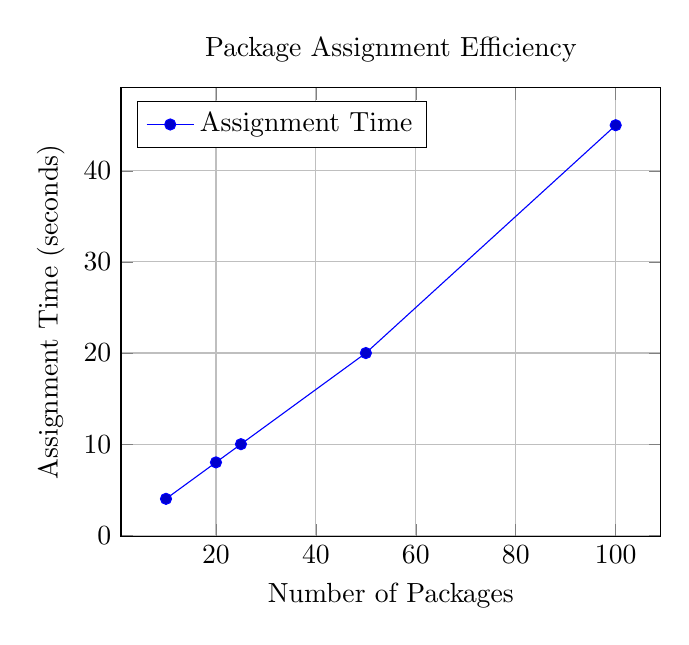
\begin{tikzpicture}
        \begin{axis}[
            title={Package Assignment Efficiency},
            xlabel={Number of Packages},
            ylabel={Assignment Time (seconds)},
            legend pos=north west,
            grid=major
        ]
        \addplot coordinates {(10,4) (20, 8) (25,10) (50,20) (100,45)};
        \addlegendentry{Assignment Time}
        \end{axis}
    \end{tikzpicture}
    \caption{Package Assignment Efficiency Analysis}
\end{figure}

% Route Optimization Performance Graph
\begin{figure}[h]
    \centering
    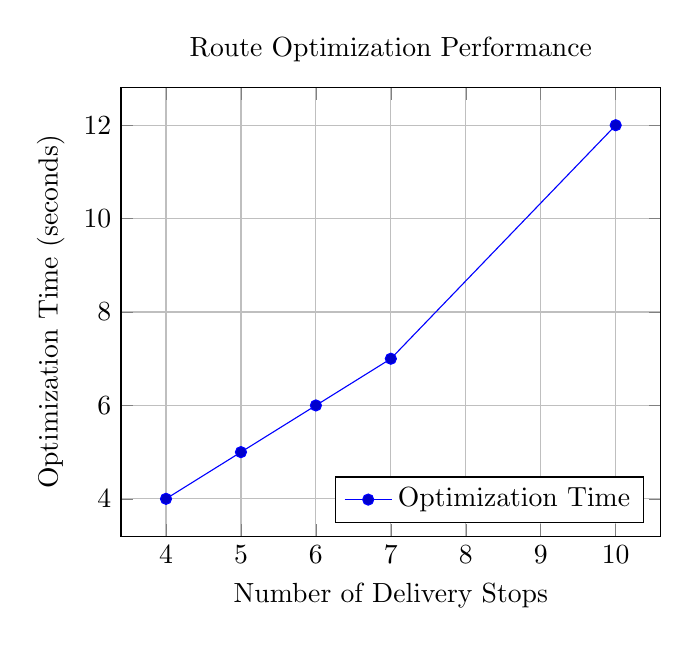
\begin{tikzpicture}
        \begin{axis}[
            title={Route Optimization Performance},
            xlabel={Number of Delivery Stops},
            ylabel={Optimization Time (seconds)},
            legend pos=south east,
            grid=major
        ]
        \addplot coordinates {(4,4) (5,5) (6,6) (7,7) (10,12)};
        \addlegendentry{Optimization Time}
        \end{axis}
    \end{tikzpicture}
    \caption{Route Optimization Performance Analysis}
\end{figure}
\section{Challenges Faced and Solution}
\subsection{Package Assignment}
\begin{itemize}
    \item Problem: The initial employee assignment algorithm only considered the total weight of packages and the vehicle’s average weight capacity. This approach often led to miscalculations, as it did not account for package size constraints or variations in real-world loading conditions. As a result, even when sufficient employees were assigned, some packages were left undelivered due to improper space utilization. Additionally, the system sometimes suggested more employees than necessary, leading to inefficiencies in workforce allocation.

    \item Solution: The algorithm was improved to factor in both weight and size constraints when calculating the required number of employees. Instead of relying solely on weight-based allocation, the system now calculates employee requirements based on both total weight and total volume.Additionally, package assignments were refined to distribute loads evenly across employees, preventing scenarios where small gaps in available space led to undelivered packages. This enhancement ensures that all packages are assigned efficiently while optimizing the use of available employees and transportation capacity.
\end{itemize}
\subsection{Route Optimization}
\begin{itemize}
    \item Problem: The algorithm did not account for the final delivery location, which resulted in incomplete routes and inefficient navigation. This caused potential delays and suboptimal travel sequences for delivery personnel.
    \item Solution: The routing algorithm was refined to ensure that the final delivery location was always included as a required stop. Additionally, the logic was adjusted to dynamically optimize the route while considering real-time location changes, enhancing delivery efficiency and accuracy.
\end{itemize}
\section{Summary}
This chapter presents the results of the FastTrack system, highlighting key features and performance
analysis. The Login \& Registration Page ensures secure authentication for companies and employees
using Firebase (Figure 6.1 \& 6.2 \& 6.3). The Package \& Employee Details Page displays package
information and employee availability for efficient assignment (Figure 6.4 \& 6.5). A QR Code
Scanning Page allows employees to scan package QR codes for quick tracking and retrieval (Figure
6.6). The Route Optimization \& Navigation Page utilizes the Greedy Algorithm and Google Maps
API to generate efficient delivery routes (Figure 6.7). Performance analysis graphs show package
assignment efficiency and route optimization time, proving the system’s effectiveness (Figure 6.8 \&  6.9). Challenges, such as missing final delivery locations in routing, were resolved by refining the algorithm for accurate navigation and optimal travel sequences.